\documentclass{standalone}
\usepackage{tikz}
\usepackage{ctex,siunitx,ninecolors}
\setCJKmainfont{Noto Serif CJK SC}
\usepackage{tkz-euclide}
\usepackage{amsmath}
\usetikzlibrary{patterns, calc}
\usetikzlibrary {decorations.pathmorphing, decorations.pathreplacing, decorations.shapes}
\pgfdeclareverticalshading{pile}{100bp}{
  color(0bp)=(black);color(50bp)=(white);color(100bp)=(black)
}
\begin{document}
\small
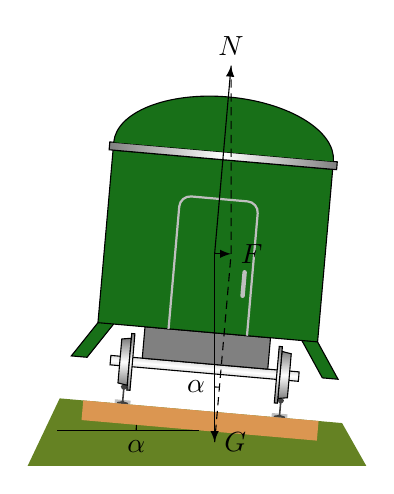
\begin{tikzpicture}[>=latex,scale=1.0]
  \fill[olive5!80!brown](-5:1.8)--(175:1.8)--(-2.2,-0.7)--(2.1,-0.7);
  \begin{scope}[rotate=-5]
  \draw[shading=pile,shading angle=-5](1.2,0.6)rectangle(-1.2,0.48);
  \foreach \x in {-1,1}
  {
    \begin{scope}[xshift=\x cm,xscale=-\x*0.2,yscale=0.2]
      \fill[lightgray](-0.5,0)rectangle(0.5,0.25);
  \fill[darkgray](0.367,0.000)..controls( 0.367,0.094)and( 0.354,0.109)..( 0.222,0.122)..controls( 0.077,0.137)and( 0.050,0.167)..( 0.050,0.195)--( 0.050,0.905)..controls( 0.050,0.933)and( 0.077,0.963)..( 0.138,0.969)..controls( 0.186,0.974)and( 0.200,0.989)..( 0.200,1.100)..controls( 0.200,1.209)and( 0.050,1.234)..( 0.000,1.234)..controls(-0.050,1.234)and(-0.200,1.209)..(-0.200,1.100)..controls(-0.200,0.989)and(-0.186,0.974)..(-0.138,0.969)..controls(-0.077,0.963)and(-0.050,0.933)..(-0.050,0.905)--(-0.050,0.195)..controls(-0.050,0.167)and(-0.077,0.137)..(-0.222,0.122)..controls(-0.354,0.109)and(-0.367,0.094)..(-0.367,0.000)--cycle;
  \fill[top color=gray,bottom color=gray,middle color=white,draw](0.2,4.2)--(0.2,1.2)--(-0.4,1.3)--(-0.4,4.1)--cycle;
  \fill[top color=gray,bottom color=gray,middle color=white,draw](0.2,0.9)rectangle(0.4,4.5);
    \end{scope}
  }
  \fill[brown7](1.5,0)rectangle(-1.5,-0.25);
  \draw[fill=gray](0.8,1)rectangle(-0.8,0.6);
  \draw[fill=green4](1.2,1)--++(0.3,-0.45)--++(0.2,0)--++(-0.3,0.45);
  \draw[fill=green4](-1.2,1)--++(-0.3,-0.45)--++(-0.2,0)--++(0.3,0.45);
  \draw[fill=green4](1.4,1)rectangle(-1.4,3.2);
  \draw[left color=gray,right color=gray,middle color=white](1.45,3.3)rectangle(-1.45,3.2);
  \draw[lightgray,rounded corners,thick](-0.5,1)--(-0.5,2.7)--(0.5,2.7)--(0.5,1);
  \draw[lightgray,ultra thick,line cap=round](0.4,1.8)--++(0,-0.3);
  \draw[fill=green4](-1.4,3.3)arc(180:0:1.4 and 0.7);
  \end{scope}
  \draw[->](85:2.0)--(85:4.4)node[above]{$N$};
  \draw[->](85:2.0)--++({2.4*sin(5)},0) coordinate (F);
  \node at (F)[right]{$F$};
  \draw[->](85:2.0)--++(0,{-2.4*cos(5)}) coordinate (G);
  \node at (G)[right]{$G$};
  \draw[thin,densely dashed](85:4.4)--(F)--(G);
  \draw[thin](265:0.25)--++(-1.8,0);
  \draw[thin]([yshift=7mm]G)arc(90:85:0.7)node[at start,left]{$\alpha$};
  \draw[thin]([xshift=-0.8cm]265:0.25)arc(180:175:0.8)node[at start,below]{$\alpha$};
\end{tikzpicture}
\end{document}